\section{User interface}
\label{sec-analyse}

The \textsf{Geant-val} website provides two ways of viewing and comparing results:

\begin{itemize}



\item \textit{Statistical comparisons} page allows comparison of simulation with compatible experimental results using a selecton of statistical tests. % It displays results of statistical comparison for pairs of plots with the same parameters' values.

In visual mode  (see Figure~\ref{fig:sc_visual_ratio}) one can select various parameters in left side drop down menu and request plots corresponding to the values selected. In this mode it is possible to choose one Geant4 release as "reference" to get ratio plots between several results.

In statistical mode (see Figure~\ref{fig:statcomparison}) the page shows results of $\chi^2$ ($\chi^2/n.d.f.$, $\chi^2$ probability) and Kolmogorov-Smirnov (KS Max(D), KS probability) tests between two Geant4 releases for all matching pairs of test results.
All computations are fast and performed asynchronously on the client side using JavaScript WebWorkers. For this purpose, JavaScript code to perform $\chi^2$ and Kolmogorov-Smirnov tests has been written, and their results cross-checked against the same statistical techniques implemented in the ROOT framework ({\tt ROOT::TH1::Chi2Test()} and {\tt ROOT:TMath::KolmogorovTest()} correspondingly).

Results are marked as ''bad'', ''warning'' and ''good'' depending on $\chi^2$ probability, exact ranges for each category can be adjusted by the user. It is also possible to download a PDF file containing the report and all plots.

\begin{figure}[h]
    \centering
    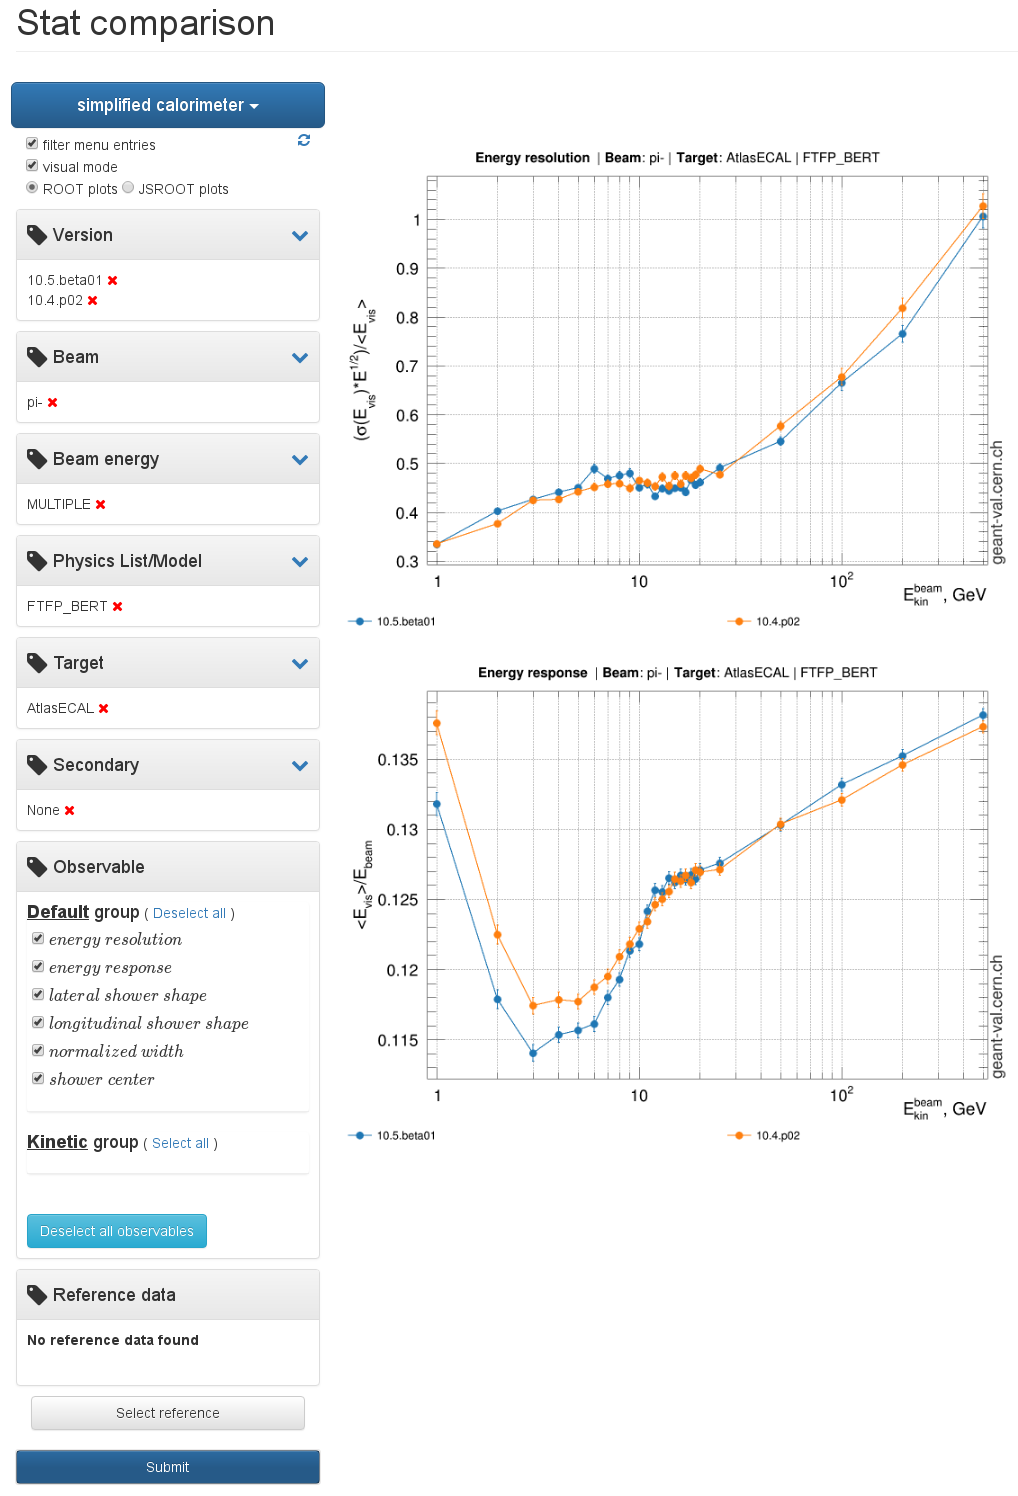
\includegraphics[width=\textwidth,clip]{sc_visual_ratio.png}
    \caption{Plots of "simplified calorimeter" test results for Geant4 releases 10.5.beta01 and 10.4.p02 with 10.5.beta01 selected as "reference".}
    \label{fig:sc_visual_ratio}
\end{figure}

\begin{figure}[h]
    \centering
    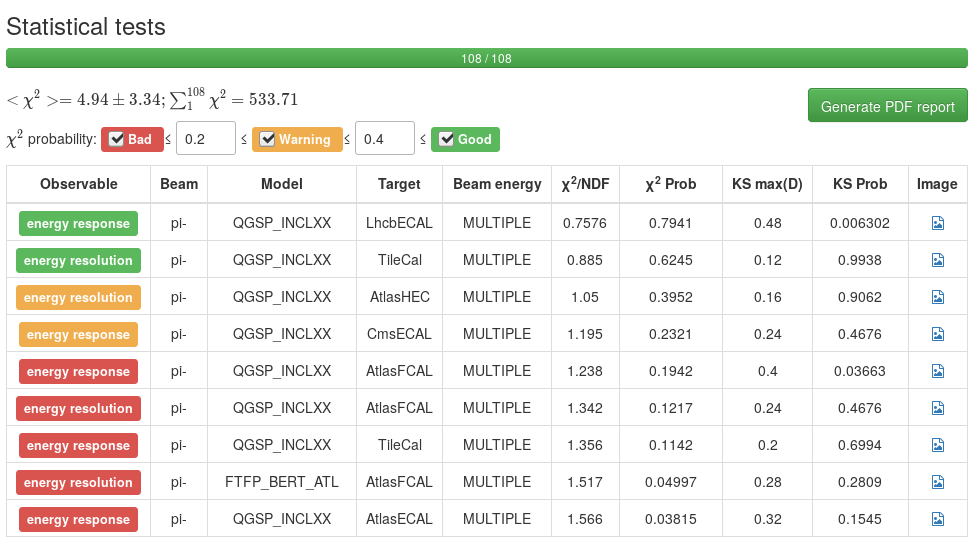
\includegraphics[width=\textwidth,clip]{statcomparison.png}
    \caption{Statistical comparison of "simplified calorimeter" test results between Geant4 releases 10.5.beta01 and 10.4.p02 for $\pi-$ beam.}
    \label{fig:statcomparison}
\end{figure}



\item \textit{User layouts} page (see Figure~\ref{fig:layouts}). A \textit{layout} is an XML file describing what plots should be displayed and how should they be laid out on a page. It can be useful for Geant4 tests that produce hundreds of different plots, whose fast "visual" validation it is often enough to compare only a small well-defined subset of them.

The user selects the desired layout, Geant4 version(s), physics list(s) and experimental data. All other plot parameters should be defined in \textit{layout} file. It allows performing fast visual comparison of several Geant4 versions/physics lists. It is also possible to produce ratio plots to better visualise the differences between different distributions.

Layouts are available "out of the box" for some tests, however users can define and use on their own layout on the website.

\begin{figure}[h]
    \centering
    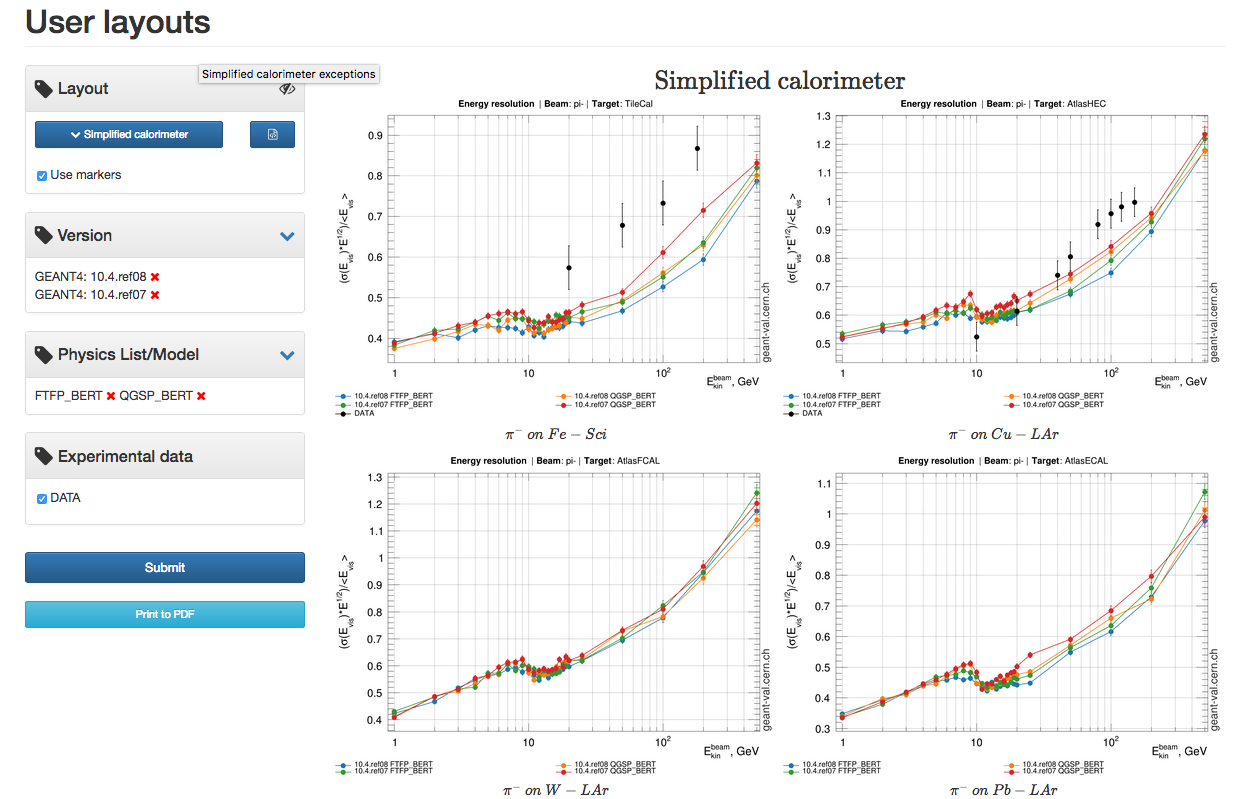
\includegraphics[width=\textwidth,clip]{layout_sc.png}
    \caption{Layout for the Geant4 "simplified calorimeter" test with results for Geant4 reference releases 10.4.ref07, 10.4.ref08 and physics lists FTFP\_BERT and QGSP\_BERT.}
    \label{fig:layouts}
\end{figure}

\end{itemize}

%In both comparison modes users can change plot's axes ranges/scales and download them in PNG, EPS, ROOT formats. Raw plot's data in Gnuplot and the website's JSON formats are also accessible.